% !TEX encoding = UTF-8 Unicode
% ------------------------------------------------------------------------------
% Este fichero es parte de la plantilla LaTeX para la realización de Proyectos
% Final de Grado, protegido bajo los términos de la licencia GFDL.
% Para más información, la licencia completa viene incluida en el
% fichero fdl-1.3.tex

% Copyright (C) 2012 SPI-FM. Universidad de Cádiz
% ------------------------------------------------------------------------------

Las instrucciones de uso del sistema se detallan a continuación.

\section{Introducción}

Este es un sistema de gestión para un centro deportivo, desarrollado concretamente para \textit{CoreSport}, centro para la mejora de la salud y el rendimiento. \\

La aplicación web será accesible desde cualquier dispositivo con conexión a internet y un navegador web, distinguiéndose 3 tipos de usuarios: superadministrador, administrador y usuario. Los socios de la empresa, y trabajadores si se estima oportuno, serán los administradores, mientras que los usuarios serán los clientes del centro. El rol de superadministrador será llevado a cabo por la persona encargada del sistema, en este caso el propio alumno desarrollador del proyecto. 


\section{Características}

Este sistema de gestión proporciona numerosas características que a continuación se detallan: 

\begin{itemize}
\item Los usuarios, administradores y superadministradores podrán realizar las siguientes acciones: 

\begin{itemize}
\item Seleccionar idioma.
\tiem Registrarse en el sistema\footnote{Todo nuevo registro se dará de alta como "usuario", si se tratase de un administrador, será asignado como tal por el superadministrador u otro administrador}.
\tiem Iniciar y cerrar sesión.
\tiem Recuperar la contraseña en caso de olvido.
\tiem Cambiar su contraseña y el resto de sus datos del perfil.
\tiem Mandar y leer correo interno.
\tiem Ver notificaciones del sistema.
\tiem Reservar plaza en una clase y cancelar las reservas.
\tiem Solicitar citas de algún servicio específico, así como cancelar la solicitud o reserva de cita.
\tiem Consultar las reservas realizadas.
\tiem Ver el calendario de actividades con todas las disponibles, las pasadas y las reservadas.
\tiem Ver el histórico de acciones realizadas en el sistema.
\tiem Ver los comunicados.
\tiem Descargarse los archivos a los que tenga acceso. 
\end{itemize}

\item Respecto a administradores y superadministardores, además de estas funcionalidades, podrán: 

\begin{itemize}
\item Responder a solicitudes de cita.
\item Cancelar la cita de un usuario.
\item Activar, suspender y editar usuarios.
\item Activar o suspender a otro administrador.
\item Ver el histórico de acciones de los usuarios del sistema y otros administradores.
\item Dar de alta, editar, suspender o activar servicios.
\item Dar de alta, editar, suspender o activar clase.
\item Dar de alta, editar, suspender o activar cita.
\item Crear nuevo, editar, asignar destinatarios o eliminar archivo.
\item Crear nuevo, editar, suspender o activar comunicado.
\end{itemize}

\item El superadministrador, además, podrá:

\begin{itemize}
\item Activar, suspender o editar administradores.
\end{itemize}

\end{itemize}


\section{Requisitos previos}

Para la utilización del sistema no se requiere ningún elemento hardware o software fuera de lo común. Cualquier dispositivo con conexión a internet y navegador web puede hacer uso de ella. 


\section{Uso del sistema}

El sistema no precisa de conocimiento fuera de lo común en un sistema de gestión. La interfaz es intuitiva y las funcionalidades están estructuradas de manera sencilla a través del menú. Se irá relatando cómo realizar las tareas disponibles, mostrando visualmente algunos ejemplos más representativos. \\

La interfaz del sistema aparecerá en el idioma por defecto de la organización, en este caso será el español. Si no hablamos castellano, se podrá \textbf{cambiar el lenguaje} haciendo uso del selector destinado a ello en la esquina superior derecha de la interfaz.

El primer paso para usar la aplicación web sería el \textit{registro de usuario}. Para ello, hacemos clic en el enlace "\textit{¿Todavía no tienes tu cuenta CoreSport? Click aquí}" que aparece bajo los campos de datos de inicio de sesión. En esta página de registro, introduciremos, al menos, los cambios obligatorios marcados con asterisco (*) y marcaremos la casilla de haber leído y aceptar los términos y condiciones, una vez hecho. Introduciendo las palabras del \textit{captcha} de seguridad podremos pasar a registrarnos haciendo clic en el botón de registro. En cuanto uno de los administradores acepte la solicitud de registro, el usuario quedará activo en el sistema y podrá hacer uso de él. \\

Para \textbf{identificarse en el sistema}, simplemente introduciremos nuestro correo electrónico y contraseña en los campos destinados a ello y pulsaremos el botón de inicio de sesión. Una vez verificados los datos el sistema nos redirigirá a la página de bienvenida. En esta página podremos ver los \textbf{comunicados} para usuarios. \\

Las posibles opciones principales para un usuario identificado, como se ha descrito en la sección anterior, serían: gestión de clases, citas, mensajes internos y datos del usuario, ver acciones realizadas, comunicados y notificaciones y consultar archivos si posee alguno para su descarga. El menú guiará al usuario por estas funcionalidades, dividiéndose en varios bloques: 

\begin{itemize}
\item Inicio
\item Reservas

\begin{itemize}
\item Calendario
\item Servicios
\item Clases
\item Citas
\item Mis Resevas
\end{itemize}

\item Mi Cuenta

\begin{itemize}
\item Perfil
\item Cambiar Contraseña
\item Correo Interno
\item Notificaciones
\item Archivos
\item Histórico de Acciones
\item Cerrar Sesión
\end{itemize}

\item Ayuda

\begin{itemize}
\item Contacto
\item Términos y Condiciones
\item About
\end{itemize}

\end{itemize}

La mayoría de las funciones son triviales y de fácil realización. Al acceder a páginas como \textbf{servicios, clases, citas, reservas, correo o archivos}, todas ellas mostrarán un cuadro con la lista de información que buscas, cada fila corresponderá a un/a servicio, clase, cita, reserva, correo o archivo, con la diferencia de que cada tabla te permitirá realizar distintas opciones con la información mostrada. \\

\begin{figure}
\centering
  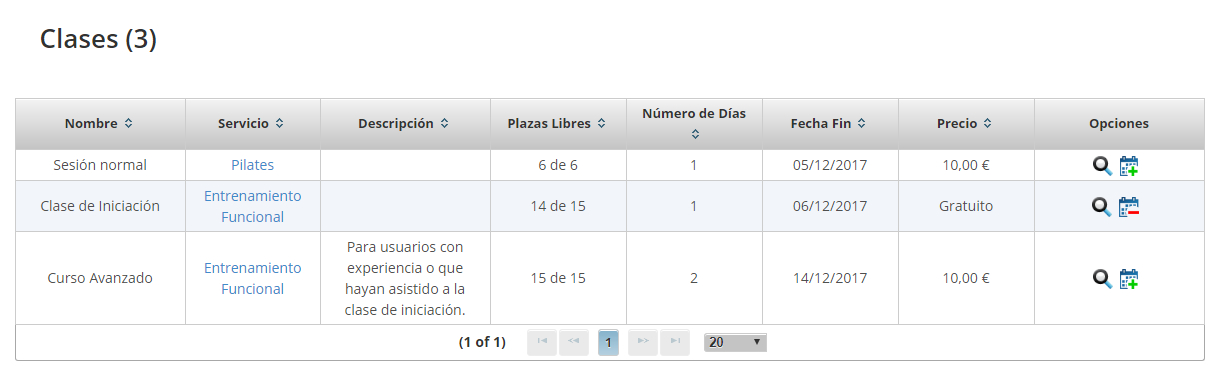
\includegraphics[scale=.70]{img/manual/tabla-clases.jpg}
  \caption{\textit{Tabla de clases}}
  \label{fig:tabla-clases}
\end{figure}

En el caso de servicios, no se permite ninguna opción a realizar. \\

Las tablas de clases y citas mostrarán la opción de ver más información detallada o reservar la clase o cita: en el primer caso, se podrá ver las plazas disponibles restantes como muestra la figura \ref{fig:tabla-clases}; en el segundo caso, cada cita mostrará su estado, que podrá ser \texit{disponible, reservada, pendiente} o \texit{suspendido/a}, como vemos en la imagen \ref{fig:tabla-citas}. Además, los estados que se muestren de color verde (\textit{aceptada}) o naranja (\textit{pendiente}) indicarán que la cita está reservada o solicitada -respectivamente- por el usuario. En cuanto a las citas pendientes, el usuario recibirá una notificación en el momento que se responda a la misma, ya sea de aceptación o rechazo. \\

Las reservas mostrarían las clases y citas del usuario -con las mismas opciones citadas-, junto con un historial de las reservas anteriores. \\

En el caso de los archivos, la opción posible será la de descarga del mismo. 

\begin{figure}
\centering
  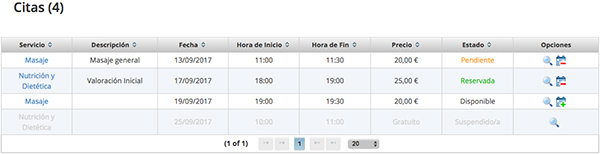
\includegraphics[scale=.70]{img/manual/tabla-citas.jpg}
  \caption{\textit{Tabla de citas}}
  \label{fig:tabla-citas}
\end{figure}

Finalizando con las páginas de tablas, el caso del correo interno sería algo diferente, ya que posee dos pestañas, una para el correo recibido (\textit{bandeja de entrada} y otra para el enviado. En este caso, y en ambas pestañas, clicando en el asunto de un correo específico se podrá acceder a la información del mismo. Se distinguirá entre nuevo correo y leído por el texto en negrita de los nuevos, como apreciamos en la imagen \ref{fig:correo-interno}. Observamos también que se da la opción a redactar un email, acción que redirigirá al usuario a la página de redacción de un nuevo email, donde elegirá el destinatario a través del desplegable que se facilita y podrá escribir el asunto y mensaje a enviar como vemos en la imagen. 

\begin{figure}
\centering
  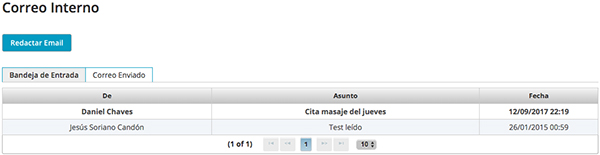
\includegraphics[scale=.70]{img/manual/correo-interno.jpg}
  \caption{\textit{Correo interno}}
  \label{fig:correo-interno}
\end{figure}

\begin{figure}
\centering
  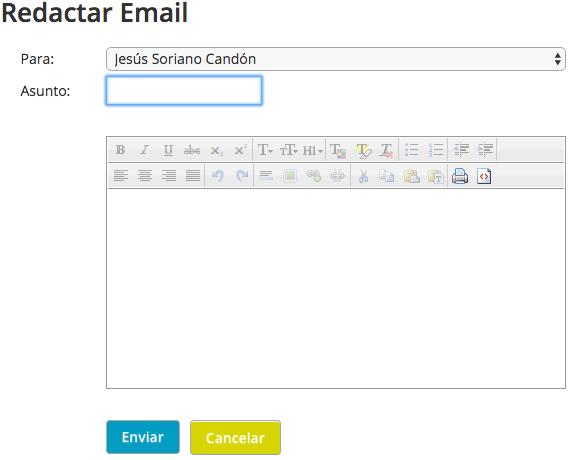
\includegraphics[scale=.50]{img/manual/redactar-email.jpg}
  \caption{\textit{Redactar email}}
  \label{fig:redactar-email}
\end{figure}

El caso de notificaciones e historial de acciones se diferencia del resto de tablas en que se eligen las fechas entre las que se desea ver la información. Las página de notificaciones mostrará todas las de la última semana, pudiendo elegir las fechas y el tipo de notificación que se desea consultar. Al igual que en el caso de los correos, las que no han sido leídas se mostrarán en negrita, quedando marcada como leída una vez vista. En cuanto al histórico de acciones, no se mostrará la tabla por defecto, sino que el usuario será el que elija las fechas y el tipo de acción a mostrar, obteniendo lo resultados definidos. \\

Otra de las opciones disponibles, y unas de las más importantes del sistema, sería el calendario de actividades. Este mostrará todas las clases y citas existentes, tanto pasadas como futuras, para una mayor facilidad de visión y ubicación en el tiempo. El calendario, como vemos en la figura \ref{calendario}, distinguirá entre citas y clases dependiendo del diseño del cuadro de información, como aclara la explicación de colores y formas que se facilita bajo el mismo. Así, vemos que las clases tendrán un fondo a color, mientras que las citas solo un borde. Los colores indicarán la misma información, si la clase o cita es pasada (gris), está disponible para reservar (azul), está reservada por el usuario (verde) o no está disponible (naranja). En este último caso, podría ser una cita en estado de \textit{pendiente}, ya sea del usuario en concreto o de cualquier otro usuario. 

\begin{figure}
\centering
  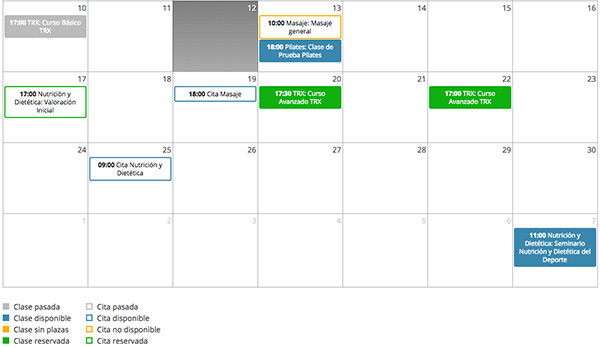
\includegraphics[scale=.60]{img/manual/calendario.jpg}
  \caption{\textit{Calendario de actividades}}
  \label{fig:calendario}
\end{figure}

Por último, la opción restante sería el perfil del usuario. Aquí, se podría ver la información del usuario junto con sus reservas. La página del perfil te permite navegar hasta la edición del mismo para modificar algunos de los datos, teniendo en cuenta que el correo electrónico es el único campo que no se podría editar. También se podrá cambiar la contraseña en la página destinada a ello.\\

No podemos olvidar que administrador y superdaministrador disponen de las mismas opciones que los clientes del centro. Por supuesto, posee muchas más, teniendo la posibilidad de crear, editar, activar y suspender servicios, clases, citas, usuarios... El menú de un administrador quedaría como sigue:

\begin{itemize}
\item Inicio
\item Reservas

\begin{itemize}
\item Calendario
\item Mis Resevas
\end{itemize}

\item Administración

\begin{itemize}
\item Usuarios
\item Administradores
\item Servicios
\item Clases
\item Citas
\item Archivos
\item Comunicados
\item Histórico de Acciones
\end{itemize}

\item Mi Cuenta

\begin{itemize}
\item Perfil
\item Cambiar Contraseña
\item Correo Interno
\item Cerrar Sesión
\end{itemize}

\item Ayuda

\begin{itemize}
\item Contacto
\item Términos y Condiciones
\item About
\end{itemize}

\end{itemize}

El del superadministrador sería prácticamente el mismo, con la diferencia de poseer una opción más en la administración, dedicada a las organizaciones, así como permisos para editar administradores.\\

A continuación vamos a ver cómo gestionar el sistema por parte los administradores. \\

Empezaremos por los servicios, que será lo primero que crearemos, necesario para clases y citas. Para ello, navegaremos hasta la página de servicios, donde vemos la opción de añadir un nuevo servicio. La gestión de estos es fácil, ya que solo tendremos que introducir el nombre (único de cada servicio) y una descripción opcional para crearlos, como vemos en la imagen \ref{fig:nuevo-servicio}. Una vez creado, se podrá editar o desactivar (y activar) el servicio. Hay que tener en cuenta que a la hora de desactivar un servicio, este puede tener clases o citas vigentes. Se suspenderá solo el servicio, y no las clases o citas vigentes; para lograr esto, se deberán suspender las mismas individualmente. 

\begin{figure}
\centering
  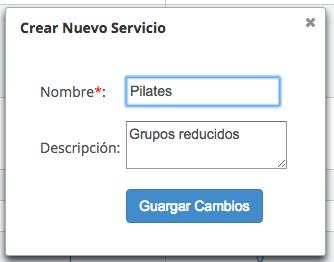
\includegraphics[scale=.70]{img/manual/crear-nuevo-servicio.jpg}
  \caption{\textit{Creación de un nuevo servicio}}
  \label{fig:nuevo-servicio}
\end{figure}

En cuanto a las clases y citas, al navegar a sus respectivas vistas, los administradores dispondrán de una tabla más que los usuarios, el historial de clases o citas. Esto puede ser valioso para consultar alguna clase o cita pasada o para crear nuevas a partir de ellas, con la opción de duplicar que ofrecen las tablas, que copiará la información de clase sin fechas o la cita asignándole la fecha del día siguiente al actual a la misma hora que la original; fechas que serán editables, claro está. En el caso de citas, existirá una opción extra en las filas de las citas que estén pendiente de respuesta de solicitud, que podremos aceptar o rechazar, como vemos en la imagen \ref{fig:tabla-citas-admin}. \\

\begin{figure}
\centering
  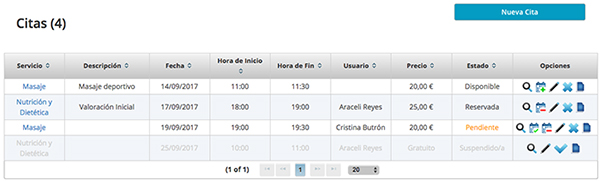
\includegraphics[scale=.70]{img/manual/tabla-citas-admin.jpg}
  \caption{\textit{Tabla de citas para el administrador}}
  \label{fig:tabla-citas-admin}
\end{figure}

Vamos observando en las tablas que cada vez aparecen más opciones en la columna de opciones y, por tanto, más iconos. La figura \ref{fig:explicacion-iconos} aporta una breve explicación de los posibles iconos que pueden aparecer en la columna de acciones de la aplicación. 

\begin{figure}
\centering
  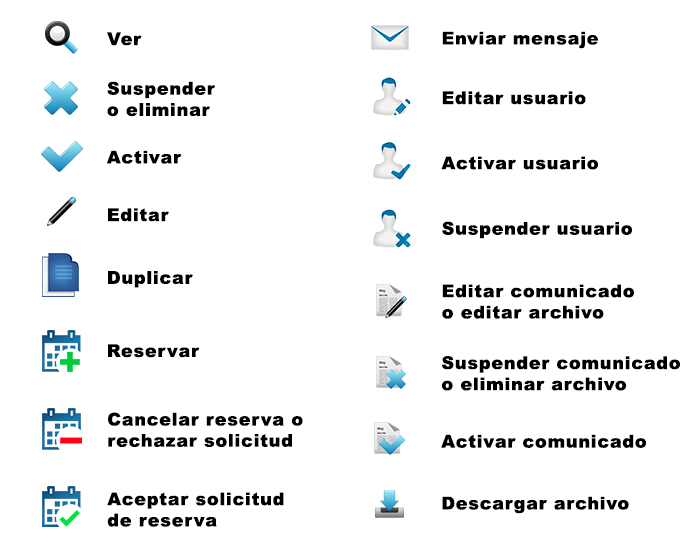
\includegraphics[scale=.50]{img/manual/explicacion-iconos.jpg}
  \caption{\textit{Breve explicación de los iconos de acción}}
  \label{fig:explicacion-iconos}
\end{figure}

Para crear clases o citas, en cada una de sus correspondientes páginas aparece un botón con tal objetivo, que llevará al administrador a la página de creación de una nueva clase o cita. Se rellenarán los campos pedidos respecto a la clase (\textit{servicio, nombre, descripción (opcional), plazas totales} y \textit{precio}) o cita (\textit{servicio, descripción (opcional), precio, fecha, hora de inicio} y \textit{hora de fin}) y se pulsará en el botón para crearla. \\

En el caso de las clases, vemos que por el momento no tendría fecha. Una vez creada una clase, es el momento de asignarle al menos una fecha. Para ello, en la vista de la clase se observa una tabla llamada \textit{Horarios}. Justo debajo aparece la opción de \textit{+ Añadir Día}. Clicando, aparecerá una pequeña ventana para añadir la fecha y hora de inicio y fin, junto con una descripción opcional del día. Para una misma clase se pueden añadir tantos días como se desee. Lo lógico, en principio, sería que cada clase posea un solo día, pero es posible que tengan más, como puede ser el caso de cursos de varios días por ejemplo. El usuario reservará plaza para la clase completa, es decir, para todos los días, no para días individuales. En caso que se desee ofrecer esta opción, habría que crear diferentes clases, cada una con un día, las cuales podrán ser reservadas de forma independiente. \\

Al igual que la tabla de días, en la vista de cada clase individual aparece una tabla de usuarios con reserva de la clase. El administrador tiene la opción de añadir clientes a la tabla, asignándole una plaza, seleccionándolo de la lista que aparece bajo la tabla y haciendo uso de la opción \textit{+ Añadir Participante}. Podemos ver un ejemplo en la figura \ref{fig:horarios-y-usuarios-clase}. De igual modo, las vistas de citas tendrán una tabla con el historial de solicitudes y aparecerá la opción de asignarle la cita a un usuario de la misma forma, en caso que la cita esté disponible. \\

\begin{figure}
\centering
  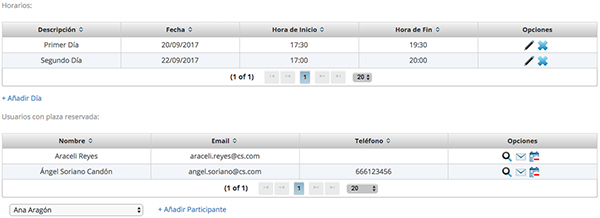
\includegraphics[scale=.60]{img/manual/horarios-y-usuarios-clase.jpg}
  \caption{\textit{Horarios y usuarios con plaza en una clase.}}
  \label{fig:horarios-y-usuarios-clase}
\end{figure}

En cuanto a la gestión de usuarios, podremos ver o editar su perfil, suspender o activar al usuario o mandarle un mensaje interno. También aparecerá la opción de añadir nuevo usuario. En este caso, el registro lo realizará directamente el administrador y el usuario recibirá un email con la confirmación de cuenta. Será una opción socorrida cuando algún cliente no registrado quiera reservar una cita o clase personándose en el centro, así como para clientes que no tenga habilidades informáticas para tal fin. \\ 

Si hablamos de la gestión de otros administradores, un administrador podrá ver su perfil o enviarle un mensaje. \\





\begin{figure}
\centering
  \includegraphics[scale=.70]{img/manual/.jpg}
  \caption{\textit{}}
  \label{fig:}
\end{figure}


\begin{figure}
\centering
  \includegraphics[scale=.70]{img/manual/.jpg}
  \caption{\textit{}}
  \label{fig:}
\end{figure}






